
O sistema eletrônico desenvolvido parte do princípio de que vários sensores podem ser utilizados para efetuar mensurações diversas, tornando a plataforma além de otimizada para a vigilância de áreas de risco, flexível inclusive para  coleta de estatísticas climáticas do local. A disposição interna dos componentes é similar a de um nanosatélite 9U, ou seja, PCBs empilhadas em um stack. A disposição interna de uma estrutura de nanosatélite 6U pode ser visualizada na figura \ref{img:nanosatelite}:

	\begin{figure}[H]
		\centering
		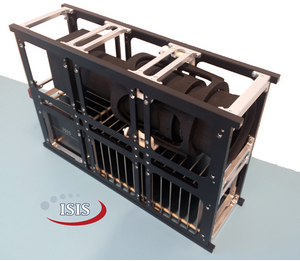
\includegraphics[width=0.5\textwidth]{figuras/nano}
		\caption{Estrutura para nanossatélite 6U ISIS }
		\label{img:nanosatelite}
	\end{figure}

\subsubsection{Áreas Contempladas} % (fold)
\label{sub:_reas_contempladas}

\subsubsubsection{Telemetria}

	A telemetria, sendo uma tecnologia que viabiliza o monitoramento, a medição ou rastreamento de uma coisa através de dados, funcionará perfeitamente para o que o projeto busca que é manter o balão sobrevoando a universidade realizando o monitoramento e ao mesmo tempo fazendo a coleta de dados sobre temperatura, umidade e também sobre alguma irregularidade na área. Essa tecnologia normalmente é feita com transmissão cabeada que possui em media 30m, ou seja, não serviria para o projeto pois possui grande risco em perda de dados pois o balão permanecerá em uma altura superior a 30m, o outro método é a transmissão sem fio (via rádio ou satélite), no caso do projeto, balão cativo, a comunicação será feita desta forma (via rádio). Existe o monitoramento em tempo real e via datalog que os dados são salvos em um cartão SD ou em pen drive, no caso do projeto o monitoramento será feito em tempo real com tempo pré determinado.
	
	Uma aplicação bastante utilizada da telemetria, é em balões meteorológicos desde o ano de 1920. Nesse ramo, o grande destaque é a comunicação sem fio utilizando o \textbf{SMS Relay}, que pode ser observado na figura \ref{img:telemetria}.

	\begin{figure}[H]
		\centering
		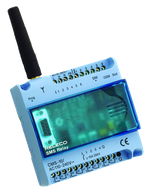
\includegraphics[width=0.3\textwidth]{figuras/telemetria}
		\caption{SMS Relay }
		\label{img:telemetria}
	\end{figure}

	O SMS Relay é um dispositivo que permite o monitoramento de uma infinita gama de equipamentos e sensores através de entradas analógicas ou digitais, e envia as informações coletadas através das entradas via SMS, ele possui também saídas de acionamento, que podem ser acionadas via SMS para ligar qualquer equipamento possibilitando uma infinidade de aplicações na automação e o mais importante é o único da categoria homologado pela ANATEL. Existem no mercado diversas soluções para monitorar algo remotamente, ou para acionar ou reiniciar equipamentos à distância, porém muitas delas não são aplicáveis na maioria das aplicações, ou seu custo inviabiliza um projeto ou torna seu uso proibitivo.

	Soluções de monitoramento baseadas internet móvel (GPRS) nem sempre apresentam um bom desempenho, pois a qualidade do serviço de internet móvel quase nunca é satisfatório onde se precisa monitorar. Já uma mensagem SMS consome muito menos dados do que o serviço de internet móvel e possui muito mais disponibilidade e estabilidade.

	Muitas soluções que utilizam radio-frequência para monitoramento remoto possuem um custo muito alto, além de implementação complicada e em muitos casos podem causar interferência em demais sistemas de comunicação o que pode causar multas e penalizações legais. Além disso há limitações de distância que a radio-frequência pode cobrir, mesmo com o uso de repetidoras e demais estruturas.

	Porém, segundo  o SMS Relay oferece uma solução confiável fabricada sobre os rígidos padrões europeus, projetada e homologada para o uso industrial e residencial, a um custo acessível quando comparado à outras soluções do mercado.

	Outro dispositivo que poderia ser utilizado na telemetria é o modulo GPRS(interface para transmissão de dados). Que pode ser observado na figura \ref{img:GPRS}.

	\begin{figure}[H]
		\centering
		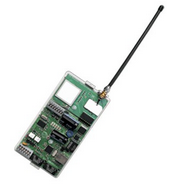
\includegraphics[width=0.3\textwidth]{figuras/GPRS}
		\caption{GPRS}
		\label{img:GPRS}
	\end{figure}

	Seguem as características do GPRS ELLO Universal:

	\begin{itemize}
		\item Atualização de Firmware remoto. 
		\item Programação via cabo USB.
		\item Reporta todos os eventos de qualquer painel de alarme que se comunique em Contact ID. 
		\item Utiliza a tecnologia GPRS para comunicação. 
		\item Saídas PGM que podem ser acionadas remotamente via GPRS.
		\item Não interfere na programação remota do painel via download.
		\item Programação realizada por software disponibilizado gratuitamente pela PPA.
		\item Supervisão anti-sabotagem e funcionamento do painel.
		\item Permite o envio de teste periódico por linha fixa. 
		\item Possui detector de corte de linha telefônica - Permite o uso em locais onde não existe linha fixa. 
	\end{itemize}
	% subsection _reas_contempladas (end)

\subsubsection{Sistemas de Telecomunicações}

\subsubsection{Controle e Automação}

Embora que a princípio o balão trabalhará com altitude fixa, este tem o grais de liberdade para mudar de orientação em torno dos eixos Z\textit{b}, Y\textit{b} e X\textit{b} (considera-se o sistema de referência Body Axes). O sistema de referência nos eixos do corpo tem origem geralmente no centro de massa, e utilizada para referenciar aeronaves, neste caso será aplicado à payload do balão. Estas mudanças de orientação ocasionarão rotações involuntárias de câmeras embarcadas no balão, dessa forma faz-se necessária a estabilização do movimento. O Sistema de Referência pode ser observado na figura \ref{img:sistReferencia}.

	\begin{figure}[H]
		\centering
		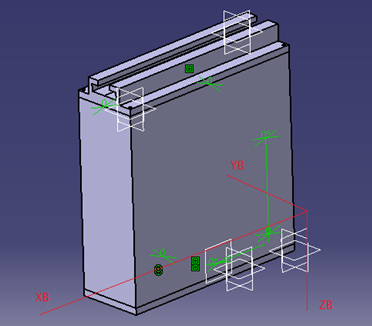
\includegraphics[width=0.5\textwidth]{figuras/sistReferencia}
		\caption{Sistema de Referência}
		\label{img:sistReferencia}
	\end{figure}

Tal movimento de rotação pode ser induzido pelas forças aerodinâmicas que agem no balão quando o fluxo de ar faz-se presente. O sistema de controle que seria capaz de estabilizar o sistema frente a uma perturbação seria classificado como de malha fechada, isso significa que um conjunto de sensores inerciais (acelerômetro, giroscópio) deve ser empregado para além de detectar a perturbação, verificar se o sistema de controle está sendo efetivo. Dessa forma o sistema de controle de malha fechada verifica se a saída condiz com as especificações de estabilidade do sistema, para se ter certeza de que a estabilização está sendo feita. O sistema de controle atuaria de forma intermitente enquanto a estabilização não fosse bem sucedida. Para fins de viabilidade, o sistema de controle empregado deve ser capaz de estabilizar a payload (setor de equipamentos embarcados) rapidamente, para se ter qualidade nas imagens geradas pela câmera.

Um provável atuador para o eixo ZB, ou seja, mecanismo capaz de efetuar a estabilização seria um Reaction Wheel. Um Reaction Wheel é um dispositivo frequentemente utilizado para o controle de atitude de satélites, consiste de um disco massivo acoplado a um eixo giratório. O princípio que o dispositivo usa para efetuar a estabilização é o momento de inércia do disco, dependendo da interpretação do algoritmo de controle das leituras dos sensores, sua rotação é ativada com velocidade e sentido determinados, executando-se a estabilização (anula a rotação da payload do balão no eixo). Tal atuador se encontrará no interior da payload. Como pode ser visto na figura \ref{img:reaction}.

	\begin{figure}[H]
		\centering
		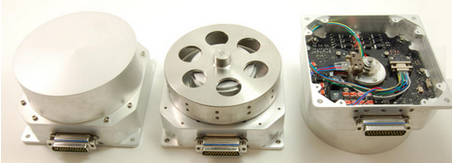
\includegraphics[width=0.5\textwidth]{figuras/reaction}
		\caption{Reaction Wheels Clyde Space}
		\label{img:reaction}
	\end{figure}

	A especificação dos Reaction Wheels comerciais da compania Clyde Space se encontra na figura \ref{img:especificacao}.

	\begin{figure}[H]
		\centering
		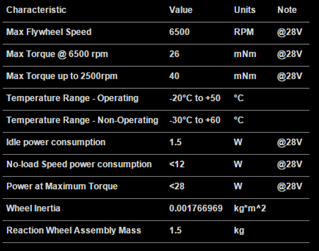
\includegraphics[width=0.5\textwidth]{figuras/especificacao}
		\caption{Especificação de Reaction Wheels Clyde Space}
		\label{img:especificacao}
	\end{figure}

	Para a estabilização do eixo YB pode ser utilizado um trilho para mover a posição da bexiga, e dessa forma alterar o ângulo de pitch, de forma a nivelar o plano seccional horizontal da payload com o solo. Tal trilho está indicado na estrutura conceitual da payload, figura \ref{img:trilho}. 

	\begin{figure}[H]
		\centering
		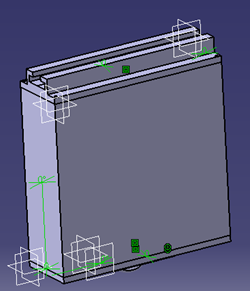
\includegraphics[width=0.5\textwidth]{figuras/trilho}
		\caption{Representação conceitual da payload, trilho em destaque.}
		\label{img:trilho}
	\end{figure}

	No caso o eixo X\textit{b}, a estabilização pode ser feita através da variação da altitude do balão em intervalos de distância pré-definidos. Essa variação da altitude pode ser feita através da retração e liberação do cabo na carretilha em solo. A instabilidade no eixo Z\textit{b} não afetará significativamente a qualidade da imagem, desde que a estabilização nos outros dois eixos seja efetiva. 

	Uma provável automação efetuada pelo balão será a avaliação de sua própria segurança. Por meio de sensores de tensão no cabo (dinamômetro) preso na estrutura da figura 5, se esta aumentar acima de um nível critico, este será automaticamente recolhido por meio do rotor motorizado em solo, e a estação de solo será informada. Assim que o sensor em solo sinalizar normalidade na velocidade do vento este será novamente elevado.

	\begin{figure}[H]
		\centering
		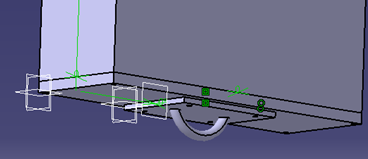
\includegraphics[width=0.5\textwidth]{figuras/parteInferior}
		\caption{Representação conceitual da parte inferior da payload, destinada à anexação do fio preso ao solo.}
		\label{img:parteInferior}
	\end{figure}

	Mais uma automação essencial será a sua elevação e retração automática para o período de monitoração determinada.